\documentclass[11pt]{article}
\usepackage[margin=1in]{geometry}
\usepackage[T1]{fontenc}
\usepackage{lmodern}
\usepackage{amsmath,amssymb,booktabs,graphicx,caption,microtype}
\usepackage[hidelinks]{hyperref}
\usepackage{xurl}
\usepackage[numbers,sort]{natbib}
\newcommand{\EOneRThreeA}{0.937}
\newcommand{\EOneNullThreeA}{0.237}
\newcommand{\EOneRThreeB}{0.969}
\newcommand{\EOneNullThreeB}{0.254}
\newcommand{\EOneRFourA}{0.847}
\newcommand{\EOneNullFourA}{0.242}
\newcommand{\HOneIIA}{0.177}
\newcommand{\HOneIIALo}{0.156}
\newcommand{\HOneIIAHi}{0.199}
\newcommand{\HOneNullQ}{0.001}
\newcommand{\HOneBranchQ}{0.000}
\newcommand{\HOneP}{0.0005}
\newcommand{\HOneEff}{0.410}
\newcommand{\HOneEffLo}{0.400}
\newcommand{\HOneEffHi}{0.420}
\newcommand{\HOneEffNullQ}{0.098}
\newcommand{\HOneEffBranchQ}{0.077}
\newcommand{\HOneEffMarginLo}{0.303}
\newcommand{\HOneEffP}{0.0005}
\newcommand{\HOneCompl}{0.403}
\newcommand{\HOneAll}{1.000}
\newcommand{\HOneFisher}{0.028}
\newcommand{\HOneClean}{0.996}
\newcommand{\HOneNElig}{4574}
\newcommand{\HOneComplEff}{0.590}
\newcommand{\HOneVerdict}{falsified}
\newcommand{\HOneHolm}{--}
\newcommand{\HRidgeIIA}{0.105}
\newcommand{\HRidgeIIALo}{0.087}
\newcommand{\HRidgeIIAHi}{0.123}
\newcommand{\HRidgeNullQ}{0.000}
\newcommand{\HRidgeBranchQ}{0.000}
\newcommand{\HRidgeP}{0.002}
\newcommand{\HRidgeEff}{0.248}
\newcommand{\HRidgeEffLo}{0.242}
\newcommand{\HRidgeEffHi}{0.254}
\newcommand{\HRidgeEffNullQ}{0.106}
\newcommand{\HRidgeEffBranchQ}{0.079}
\newcommand{\HRidgeEffMarginLo}{0.136}
\newcommand{\HRidgeEffP}{0.002}
\newcommand{\HRidgeCompl}{0.019}
\newcommand{\HRidgeAll}{1.000}
\newcommand{\HRidgeFisher}{0.023}
\newcommand{\HRidgeClean}{1.000}
\newcommand{\HRidgeNElig}{4608}
\newcommand{\HRidgeComplEff}{0.753}
\newcommand{\HRidgeVerdict}{supported}
\newcommand{\HRidgeHolm}{0.004}
\newcommand{\HTwoIIA}{0.405}
\newcommand{\HTwoIIALo}{0.371}
\newcommand{\HTwoIIAHi}{0.440}
\newcommand{\HTwoNullQ}{0.054}
\newcommand{\HTwoBranchQ}{0.031}
\newcommand{\HTwoP}{0.001}
\newcommand{\HTwoEff}{0.393}
\newcommand{\HTwoEffLo}{0.387}
\newcommand{\HTwoEffHi}{0.399}
\newcommand{\HTwoEffNullQ}{0.141}
\newcommand{\HTwoEffBranchQ}{0.098}
\newcommand{\HTwoEffMarginLo}{0.243}
\newcommand{\HTwoEffP}{0.001}
\newcommand{\HTwoCompl}{0.595}
\newcommand{\HTwoAll}{1.000}
\newcommand{\HTwoFisher}{0.016}
\newcommand{\HTwoClean}{1.000}
\newcommand{\HTwoNElig}{2304}
\newcommand{\HTwoComplEff}{0.607}
\newcommand{\HTwoVerdict}{supported}
\newcommand{\HTwoHolm}{0.004}
\newcommand{\HFourIIA}{0.058}
\newcommand{\HFourIIALo}{0.045}
\newcommand{\HFourIIAHi}{0.071}
\newcommand{\HFourNullQ}{0.005}
\newcommand{\HFourBranchQ}{0.000}
\newcommand{\HFourP}{0.0005}
\newcommand{\HFourEff}{0.324}
\newcommand{\HFourEffLo}{0.314}
\newcommand{\HFourEffHi}{0.333}
\newcommand{\HFourEffNullQ}{0.169}
\newcommand{\HFourEffBranchQ}{0.096}
\newcommand{\HFourEffMarginLo}{0.141}
\newcommand{\HFourEffP}{0.0005}
\newcommand{\HFourCompl}{0.757}
\newcommand{\HFourAll}{1.000}
\newcommand{\HFourFisher}{0.007}
\newcommand{\HFourClean}{0.999}
\newcommand{\HFourNElig}{4597}
\newcommand{\HFourComplEff}{0.677}
\newcommand{\HFourVerdict}{supported}
\newcommand{\HFourHolm}{0.0025}
\newcommand{\HCompIIA}{0.190}
\newcommand{\HCompIIALo}{0.169}
\newcommand{\HCompIIAHi}{0.211}
\newcommand{\HCompNullQ}{0.001}
\newcommand{\HCompBranchQ}{0.001}
\newcommand{\HCompP}{0.001}
\newcommand{\HCompEff}{0.415}
\newcommand{\HCompEffLo}{0.406}
\newcommand{\HCompEffHi}{0.425}
\newcommand{\HCompEffNullQ}{0.104}
\newcommand{\HCompEffBranchQ}{0.068}
\newcommand{\HCompEffMarginLo}{0.300}
\newcommand{\HCompEffP}{0.001}
\newcommand{\HCompCompl}{0.435}
\newcommand{\HCompAll}{1.000}
\newcommand{\HCompFisher}{0.028}
\newcommand{\HCompClean}{0.995}
\newcommand{\HCompNElig}{4553}
\newcommand{\HCompComplEff}{0.586}
\newcommand{\HCompVerdict}{supported}
\newcommand{\HCompHolm}{0.004}
\newcommand{\HFiveIIA}{0.072}
\newcommand{\HFiveIIALo}{0.054}
\newcommand{\HFiveIIAHi}{0.091}
\newcommand{\HFiveNullQ}{0.000}
\newcommand{\HFiveBranchQ}{0.000}
\newcommand{\HFiveP}{0.001}
\newcommand{\HFiveEff}{0.287}
\newcommand{\HFiveEffLo}{0.264}
\newcommand{\HFiveEffHi}{0.310}
\newcommand{\HFiveEffNullQ}{0.075}
\newcommand{\HFiveEffBranchQ}{0.067}
\newcommand{\HFiveEffMarginLo}{0.187}
\newcommand{\HFiveEffP}{0.001}
\newcommand{\HFiveCompl}{0.847}
\newcommand{\HFiveAll}{1.000}
\newcommand{\HFiveFisher}{0.000}
\newcommand{\HFiveClean}{1.000}
\newcommand{\HFiveNElig}{2530}
\newcommand{\HFiveComplEff}{0.710}
\newcommand{\HFiveVerdict}{supported}
\newcommand{\HFiveHolm}{0.004}
\newcommand{\HSeedThreeIIA}{0.172}
\newcommand{\HSeedThreeIIALo}{0.151}
\newcommand{\HSeedThreeIIAHi}{0.193}
\newcommand{\HSeedThreeNullQ}{0.001}
\newcommand{\HSeedThreeBranchQ}{0.001}
\newcommand{\HSeedThreeP}{0.002}
\newcommand{\HSeedThreeEff}{0.410}
\newcommand{\HSeedThreeEffLo}{0.400}
\newcommand{\HSeedThreeEffHi}{0.420}
\newcommand{\HSeedThreeEffNullQ}{0.094}
\newcommand{\HSeedThreeEffBranchQ}{0.074}
\newcommand{\HSeedThreeEffMarginLo}{0.306}
\newcommand{\HSeedThreeEffP}{0.002}
\newcommand{\HSeedThreeCompl}{0.409}
\newcommand{\HSeedThreeAll}{1.000}
\newcommand{\HSeedThreeFisher}{0.023}
\newcommand{\HSeedThreeClean}{0.999}
\newcommand{\HSeedThreeNElig}{4600}
\newcommand{\HSeedThreeComplEff}{0.590}
\newcommand{\HSeedThreeVerdict}{falsified}
\newcommand{\HSeedThreeHolm}{--}
\newcommand{\HSeedFourIIA}{0.171}
\newcommand{\HSeedFourIIALo}{0.149}
\newcommand{\HSeedFourIIAHi}{0.193}
\newcommand{\HSeedFourNullQ}{0.001}
\newcommand{\HSeedFourBranchQ}{0.000}
\newcommand{\HSeedFourP}{0.002}
\newcommand{\HSeedFourEff}{0.407}
\newcommand{\HSeedFourEffLo}{0.397}
\newcommand{\HSeedFourEffHi}{0.416}
\newcommand{\HSeedFourEffNullQ}{0.104}
\newcommand{\HSeedFourEffBranchQ}{0.081}
\newcommand{\HSeedFourEffMarginLo}{0.294}
\newcommand{\HSeedFourEffP}{0.002}
\newcommand{\HSeedFourCompl}{0.407}
\newcommand{\HSeedFourAll}{1.000}
\newcommand{\HSeedFourFisher}{0.027}
\newcommand{\HSeedFourClean}{0.991}
\newcommand{\HSeedFourNElig}{4529}
\newcommand{\HSeedFourComplEff}{0.594}
\newcommand{\HSeedFourVerdict}{falsified}
\newcommand{\HSeedFourHolm}{--}
\newcommand{\HLrnIIA}{0.172}
\newcommand{\HLrnIIALo}{0.150}
\newcommand{\HLrnIIAHi}{0.194}
\newcommand{\HLrnNullQ}{0.000}
\newcommand{\HLrnBranchQ}{0.000}
\newcommand{\HLrnP}{0.002}
\newcommand{\HLrnEff}{0.406}
\newcommand{\HLrnEffLo}{0.397}
\newcommand{\HLrnEffHi}{0.415}
\newcommand{\HLrnEffNullQ}{0.096}
\newcommand{\HLrnEffBranchQ}{0.074}
\newcommand{\HLrnEffMarginLo}{0.302}
\newcommand{\HLrnEffP}{0.002}
\newcommand{\HLrnCompl}{0.405}
\newcommand{\HLrnAll}{1.000}
\newcommand{\HLrnFisher}{0.025}
\newcommand{\HLrnClean}{0.996}
\newcommand{\HLrnNElig}{4568}
\newcommand{\HLrnComplEff}{0.594}
\newcommand{\HLrnVerdict}{falsified}
\newcommand{\HLrnHolm}{--}
\newcommand{\HOneCloser}{0.382}
\newcommand{\HOneSham}{0.999}
\newcommand{\HOneAblFam}{0.806}
\newcommand{\HOneAblNull}{0.985}
\newcommand{\HOneAblCompl}{0.553}
\newcommand{\HTwoLineToArc}{0.807}
\newcommand{\HTwoArcToLine}{0.003}
\newcommand{\HFiveNImg}{506}
\newcommand{\HFiveAbsentEff}{0.135}
\newcommand{\HFiveAbsentIIA}{0.017}
\newcommand{\RelFlipFam}{0.172}
\newcommand{\RelFlipNull}{0.093}
\newcommand{\RelFlipQ}{0.110}
\newcommand{\RelFlipP}{0.0099}
\newcommand{\RelKLFam}{0.2054}
\newcommand{\RelKLNull}{0.0501}
\newcommand{\RelKLP}{0.0099}
\newcommand{\RelN}{1962}
\newcommand{\DoseEffOne}{0.040}
\newcommand{\DoseEffTwo}{0.080}
\newcommand{\DoseEffThree}{0.119}
\newcommand{\DoseEffFive}{0.202}
\newcommand{\DoseEffSeven}{0.285}
\newcommand{\DoseEffTen}{0.410}
\newcommand{\DoseIIAOne}{0.000}
\newcommand{\DoseIIATwo}{0.001}
\newcommand{\DoseIIAThree}{0.002}
\newcommand{\DoseIIAFive}{0.013}
\newcommand{\DoseIIASeven}{0.045}
\newcommand{\DoseIIATen}{0.177}
\newcommand{\TopKTen}{0.103}
\newcommand{\TopKTwenty}{0.359}
\newcommand{\TopKForty}{0.442}
\newcommand{\TopKEighty}{0.792}
\newcommand{\TopKOneSixty}{0.979}
\newcommand{\DThetaA}{0.111}
\newcommand{\DThetaB}{0.105}
\newcommand{\DThetaC}{0.222}
\newcommand{\DThetaD}{0.303}
\newcommand{\DThetaE}{0.149}
\newcommand{\RotPredOne}{-36}
\newcommand{\RotObsOne}{-8}
\newcommand{\HFiveIIAOneEighty}{0.140}
\newcommand{\HFiveIIAFortyFive}{0.030}

\graphicspath{{../../figures/}}
\newcommand{\iia}{\mathrm{IIA}}

\title{Counterfactual Concept Swaps on InceptionV1 Curve Detectors:\\ a Specific but Partial Causal Mediator of Curve Orientation}
\author{Libor Burian}
\date{October 2026}

\begin{document}
\maketitle

\begin{abstract}
Circuits-style neuron explanations in vision models rest mostly on observational evidence. We test one of the best-characterised, ``the ten InceptionV1 \texttt{mixed3b} units are curve detectors tuned to orientation'', with pre-registered counterfactual interchange interventions (concept swaps). After reproducing the authors' published tuning curves ($r=\EOneRThreeB$), we copy the family's activations between images that differ only in curve orientation and read the next layer's published curve units. The family is a highly \emph{specific} mediator: it moves the next layer's curve code $\HOneEff$ of the way to the source, versus a 95th percentile of $\HOneEffNullQ$ for 2000 activation-change-matched 10-channel controls. It carries curvature, flipping a line to ``arc'' in $\HTwoLineToArc$ of pairs, and its ablation changes the network's predictions on natural images about twice as often as matched ablations ($\RelFlipFam$ vs $\RelFlipNull$). It is \emph{not sufficient}: the next layer decodes the source orientation in only $\HOneIIA$ of pairs [\HOneIIALo, \HOneIIAHi], so the pre-registered strong hypothesis is falsified. The orientation code is distributed and redundant (complement interchange accuracy $\HOneCompl$; about 80 channels for reliable transfer), and effects add almost linearly. The same specific-but-partial pattern holds for the 3a$\to$3b curve circuit, on natural backgrounds, and under a natural rotation counterfactual. Post-hoc checks leave these conclusions unchanged: a stricter rank-matched null, the decoded-orientation metric, and blur-free rotations.
\end{abstract}

\section{Introduction}
Neuron-level explanations of vision models are mostly \emph{observational}. A unit is called a ``curve detector'' because it fires on curves, because its feature visualization looks like a curve, and because its weights connect to other curve-like units~\cite{olah2020zoom,cammarata2020curve,cammarata2021circuits}. In language models, \citet{huang2023rigorously} showed that even confident neuron explanations can have high observational error rates and little to no causal effect when tested \emph{interventionally}. In their test, the explanation is a causal claim that the unit mediates the concept: copying the unit's value from a source input into a base input should make the model behave as if it saw the source. Related ``concept swap'' tests now validate representations in language models: digit-position neurons~\cite{baeumel2025modular}, SAE and attribution-graph features~\cite{bricken2023monosemanticity,ameisen2025circuit}, and the Jacobian-lens workspace~\cite{gurnee2026workspace}.

We apply this interventional standard to the best-characterised neuron family in vision: the ten \texttt{mixed3b} curve detectors of InceptionV1~\cite{cammarata2020curve,gorton2024missing}. The explanation names a concrete variable, curve orientation. That makes exact counterfactual pairs possible: two images identical except for orientation. It also lets us check our setup against the authors' published tuning data before any intervention.

\paragraph{Contributions.}
\begin{itemize}
\item We reproduce the published tuning curves of the 3a, 3b and 4a curve families. The fit is $r=\EOneRThreeB$ for 3b and $r=\EOneRFourA$ for 4a, with the orientation convention fitted on 3a only (\S\ref{sec:e1}).
\item We run pre-registered interchange interventions with activation-change-matched and branch-matched null neuron sets. Readouts are the published \texttt{mixed4a} curve family and, separately, all of \texttt{mixed4a}. We also test natural images.
\item The main result is mixed. The curve family moves the next layer's orientation code $\HOneEff$ of the way to the source; 95\% of activation-change-matched 10-channel controls move it less than $\HOneEffNullQ$, and none transfers the decoded orientation in more than 0.13\% of pairs. Yet swapping the family makes the next layer decode the source orientation in only $\HOneIIA$ of pairs. By our pre-registered rule, the strong sufficiency claim is falsified. The family is a highly specific but partial mediator, and other \texttt{mixed3b} channels redundantly carry the orientation.
\end{itemize}

\section{Background and related work}
\paragraph{Circuits and curve detectors.}
\citet{olah2020zoom} introduced the circuits framing, and \citet{olah2020early} catalogued InceptionV1's early-vision families. \citet{cammarata2020curve} characterised ten \texttt{mixed3b} curve units with synthetic curves and radial tuning curves. \citet{cammarata2021circuits} reverse-engineered how 3a curves build 3b curves. \citet{olah2020equivariance} described the family as rotated copies of one feature, and \citet{voss2021branch} located curve units in the 5$\times$5 branch. \citet{gorton2024missing} found additional curve features with sparse autoencoders. \citet{cammarata2026clean} revisits layer 3b and argues that neurons are cleaner than superposition accounts suggest. None of these works runs counterfactual activation swaps on the family.

\paragraph{Evaluating neuron explanations.}
Network dissection labels units and ablates them~\cite{bau2017dissection,bau2020units}. Class selectivity does not predict ablation importance~\cite{morcos2018single,leavitt2020selectivity}, and feature visualizations can mislead~\cite{geirhos2023trust}. Synthetic-image checks~\cite{kopf2024cosy} and metric sanity checks~\cite{oikarinen2025evaluating} evaluate explanations observationally. Recent work frames unit interpretation as falsifiable hypothesis testing~\cite{colorneurons2026}.

\paragraph{Interchange interventions.}
Causal abstraction~\cite{geiger2021causal,geiger2023abstraction} formalises when a set of units realises a high-level variable. Its operational test is the interchange intervention, also called activation patching. We follow the metric advice of \citet{zhang2024patching} and \citet{heimersheim2024patching}: a binary success measure (IIA) plus a continuous, roughly linear effect. Resampling-based hypothesis tests~\cite{chan2022scrubbing} motivate our complement and null sets.

\section{Method}
\label{sec:method}
\paragraph{Model.}
We use the Lucid InceptionV1 (``inception5h''; \citealp{szegedy2015going}), loaded with Lucent. Its local response normalisation is set to the TensorFlow-exact constants (window 11, $\alpha=11\cdot10^{-4}$, $\beta=0.5$, $k=2$; Lucent PR~\#51). All convolutions run in fp32 with TF32 disabled.

\paragraph{Stimuli and splits.}
Arcs are rendered with 4$\times$ supersampling. Each spans 120$^\circ$, and its midpoint sits on the receptive-field (RF) centre of the readout units, pixel (111,111), found from the input-gradient centre of mass~\cite{luo2016erf}. The orientation $\theta$ is the direction from the midpoint to the centre of curvature. A split is 72 orientations $\times$ radii $\{30,45,60,80\}$ $\times$ widths $\{3,5\}$ $\times$ two polarities, giving 1152 images. Each nuisance cell gets one random translation of $\pm2$\,px, and the jitter seed defines the split: selection (seed 1) and confirmatory (seed 2). Each base gets four sources from its own cell with $|\Delta\theta|\ge30^\circ$, giving 4608 minimal pairs.

\paragraph{Intervention.}
The readout is \texttt{mixed4a} unit (6,6). It depends only on an $11\times11$ window of \texttt{mixed3b}: the 5$\times$5 convolution sees \texttt{maxpool4} cells 4--8, which pool \texttt{mixed3b} rows 8--18. For a neuron set $S$ we overwrite channels $S$ of the base window with the source's values and recompute \texttt{maxpool4}$\to$\texttt{mixed4a} on the window. This equals the full network to $10^{-14}$ in fp64 (unit test).

\paragraph{Readouts $\tau$ and metrics.}
The primary readout uses the 14 published \texttt{mixed4a} curve units (pre-ReLU, z-scored on the selection split). Orientation is decoded by maximum Pearson correlation with the 72 clean selection templates of the pair's nuisance cell. The interchange intervention accuracy is
\begin{equation}
\iia(S)=\frac{1}{|P|}\sum_{(b,s)\in P}\mathbf{1}\!\left[\big|\tau(M_{S\leftarrow s}(b))-\tau(M(s))\big|_{\circ}\le10^\circ\right],
\end{equation}
taken over eligible pairs $P$: those whose clean base and clean source both decode within 10$^\circ$ of their true orientation. The continuous \emph{normalized effect} is $\sum\langle z_p-z_b,z_s-z_b\rangle/\sum\lVert z_s-z_b\rVert^2$, over pairs outside the lowest 5\% of $\lVert z_s-z_b\rVert^2$. It is 0 for no change and 1 when the readout becomes the source's. The secondary, non-circular readout is a ridge regression from all 508 \texttt{mixed4a} channels to $(\cos\theta,\sin\theta)$.

\paragraph{Controls.}
A patch acts only through channels whose values differ between base and source, so a random null is too easy to beat. Our primary null draws 2000 non-family sets matched to the family's histogram over deciles of $\Delta_c$, the mean squared base$\to$source change of channel $c$ on selection pairs. A co-primary null draws 2000 sets from the rest of the 5$\times$5 branch. References are the Fisher-score top-10 channels for $\theta$~\cite{gu2011fisher,baeumel2025modular}, the complement (470 channels) and all 480 channels.

\paragraph{Statistics.}
Pairs share base and source images, so we use the pigeonhole bootstrap~\cite{owen2007pigeonhole} ($B=2000$), recomputing the null's 95th percentile in every replicate. $p$-values are $(1+\#\{\text{null}\ge\text{obs}\})/(1+M)$~\cite{phipson2010permutation}, and secondary tests are Holm-corrected.

\paragraph{Pre-registered decision rule.}
Written before the confirmatory run, with pilot results disclosed. Let $D=\iia_{\text{family}}-q_{95}(\text{null})$. H1 is \emph{supported} if $\iia\ge0.5$, $D\ge0.10$, and the 95\% CI lower bound of $D$ is above 0 against both nulls. It is \emph{falsified} if the CI upper bound of $D$ is below 0.05 or $\iia<0.2$; otherwise it is inconclusive. Each secondary hypothesis is supported if its normalized-effect margin over the $\Delta$-matched $q_{95}$ has a CI lower bound above 0 and a Holm-adjusted $p<0.05$.

\section{Results}
\label{sec:results}

\subsection{E1: the observational explanation replicates}
\label{sec:e1}
We fitted one orientation convention (a reflection plus a 180$^\circ$ shift) on \texttt{mixed3a} alone, with mean $r=\EOneRThreeA$. Under that convention, our radial tuning curves match the published ones with mean Pearson $r=\EOneRThreeB$ for the 10 \texttt{mixed3b} units (every unit between 0.96 and 0.98) and $r=\EOneRFourA$ for the 14 \texttt{mixed4a} units. The 95th percentiles of a unit-label permutation null are $\EOneNullThreeB$ and $\EOneNullFourA$, and $p=10^{-4}$ for each (Fig.~\ref{fig:e1}). Each 3b unit separates arcs within $\pm45^\circ$ of its preferred orientation from other orientations with AUROC 0.70--0.95, and from straight lines with AUROC 0.67--0.92. With Lucent's default LRN constants instead of the TF-exact ones, the correlations are essentially unchanged ($\EOneLucentRThreeB$ for 3b, $\EOneLucentRFourA$ for 4a). Our model port, renderer and readout therefore reproduce the evidence the explanation rests on.

\begin{figure}[t]\centering
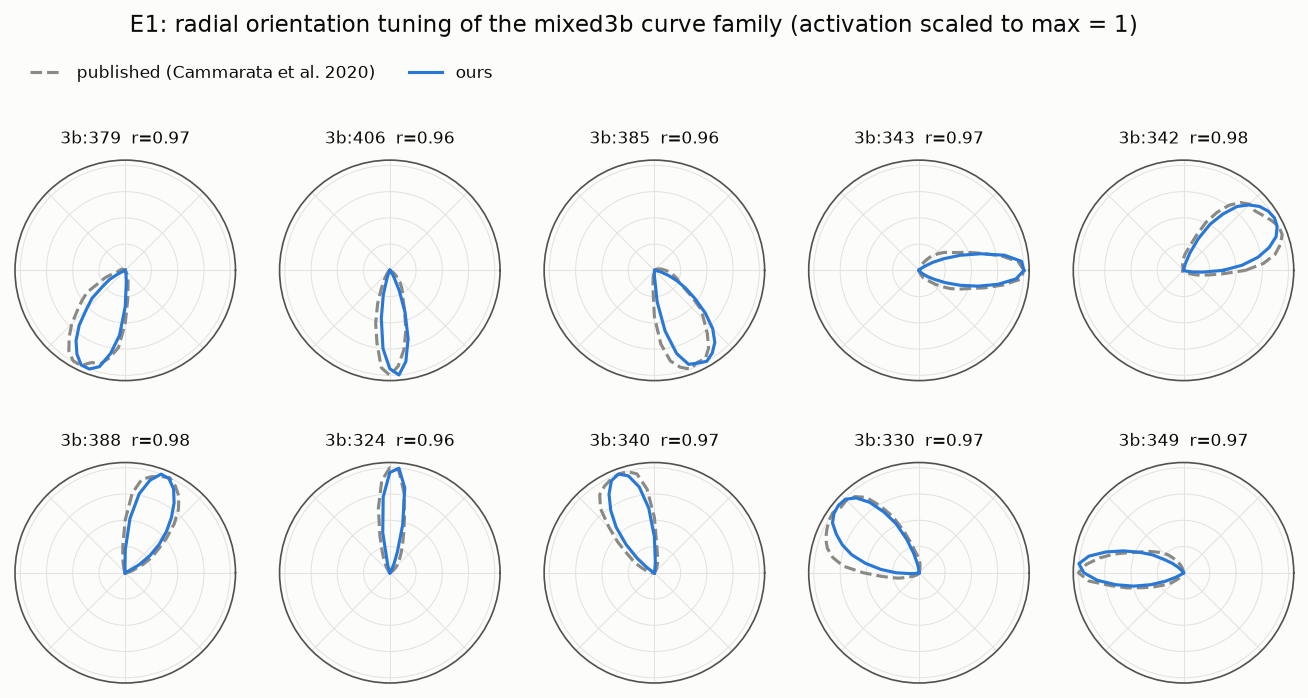
\includegraphics[width=\linewidth]{e1_radial_3b.png}
\caption{E1. Radial orientation tuning of the 10 \texttt{mixed3b} curve units: ours (blue) and published by \citet{cammarata2020curve} (gray, dashed), each scaled to a maximum of 1. The orientation convention was fitted on \texttt{mixed3a} only.}
\label{fig:e1}\end{figure}

\subsection{E2: the family is specific but not sufficient}
\paragraph{H1 (primary).}
Clean decoding accuracy is $\HOneClean$, leaving $\HOneNElig$ of 4608 pairs eligible. Swapping the 10 curve units yields $\iia=\HOneIIA$ [\HOneIIALo, \HOneIIAHi]. This is below the pre-registered falsification bound of 0.2, so \textbf{H1 is falsified}. The verdict is identical for two further jitter seeds ($\iia=\HSeedThreeIIA$, $\HSeedFourIIA$) and with Lucent's default LRN ($\HLrnIIA$).

\paragraph{Specificity.}
The same swap is far more potent than any matched control (Fig.~\ref{fig:h1}). The $\Delta$-matched null has IIA $q_{95}=\HOneNullQ$ and the branch-matched null $q_{95}=\HOneBranchQ$; across 4000 sets the best transfers orientation in 0.13\% of pairs ($p=\HOneP$ against each null). The normalized effect of the family is $\HOneEff$ [\HOneEffLo, \HOneEffHi], against a $\Delta$-matched $q_{95}$ of $\HOneEffNullQ$ and a branch-matched $q_{95}$ of $\HOneEffBranchQ$. The data-driven Fisher top-10, which shares 4 units with the family, reaches only $\iia=\HOneFisher$. Mean-ablating the family leaves the base orientation decodable in $\HOneAblFam$ of pairs, against $\HOneAblNull$ for $\Delta$-matched ablations. A same-orientation sham leaves it decodable in $\HOneSham$.

\paragraph{Redundancy and additivity.}
The 470 complementary channels reach $\iia=\HOneCompl$ and effect $\HOneComplEff$. The two effects sum to 1.000. Over random $K$-subsets of the family, the effect grows almost linearly: $\DoseEffOne,\DoseEffTwo,\DoseEffThree,\DoseEffFive,\DoseEffSeven,\DoseEffTen$ for $K=1,2,3,5,7,10$. IIA, in contrast, stays near 0 until $K=7$ ($\DoseIIASeven$) and reaches $\DoseIIATen$ at $K=10$. Additivity is partly structural: 6 of the 14 readout units belong to the $1\times1$ branch, whose pre-ReLU output is linear in the max-pooled \texttt{mixed3b} channels. Patching the top-$K$ channels by activation change gives $\iia=\TopKTwenty,\TopKForty,\TopKEighty,\TopKOneSixty$ for $K=20,40,80,160$. Reliable transfer therefore needs about 80 channels, and the 10 curve units are all among the top 17.

\paragraph{Secondary tests.}
All five secondary hypotheses meet the pre-registered criterion. The Holm-adjusted $p$-values are $\le0.004$ (Table~\ref{tab:main}; Fig.~\ref{fig:summary}).
\begin{itemize}
\item \textbf{Ridge readout over all 508 \texttt{mixed4a} channels.} This is non-circular. As pre-registered, the effect is the projection over all 508 z-scored channels: $\HRidgeEff$ against a null $q_{95}$ of $\HRidgeEffNullQ$, with $\iia=\HRidgeIIA$. It therefore measures whole-layer movement. Post hoc, we also measure it on the decoded orientation (\S\ref{sec:posthoc}).
\item \textbf{Curvature swap (H2).} The family's effect is $\HTwoEff$ against $\HTwoEffNullQ$. Inserting the family's arc activations into a line image makes the 4a curve units read ``arc'' in $\HTwoLineToArc$ of pairs. The reverse direction succeeds in only $\HTwoArcToLine$ of pairs: other channels also signal curvature.
\item \textbf{The Curve Circuits claim, 3a$\to$3b (H4).} The effect is $\HFourEff$ against $\HFourEffNullQ$. IIA is only $\HFourIIA$ while the complement reaches $\HFourCompl$, the same specific-but-partial pattern as H1.
\end{itemize}
In the exploratory analyses, IIA depends on the orientation difference: $\DThetaA$ for $|\Delta\theta|$ in 30--60$^\circ$ and $\DThetaD$ in 120--150$^\circ$. A J-lens/SAE-style \emph{family rotation} swap gives each unit the map of its neighbour on the orientation circle. It shifts the decoded orientation in the predicted direction, but by only 21--39\% of the predicted angle (e.g.\ $\RotObsOne^\circ$ vs $\RotPredOne^\circ$ for $k=1$).

\begin{figure}[t]\centering
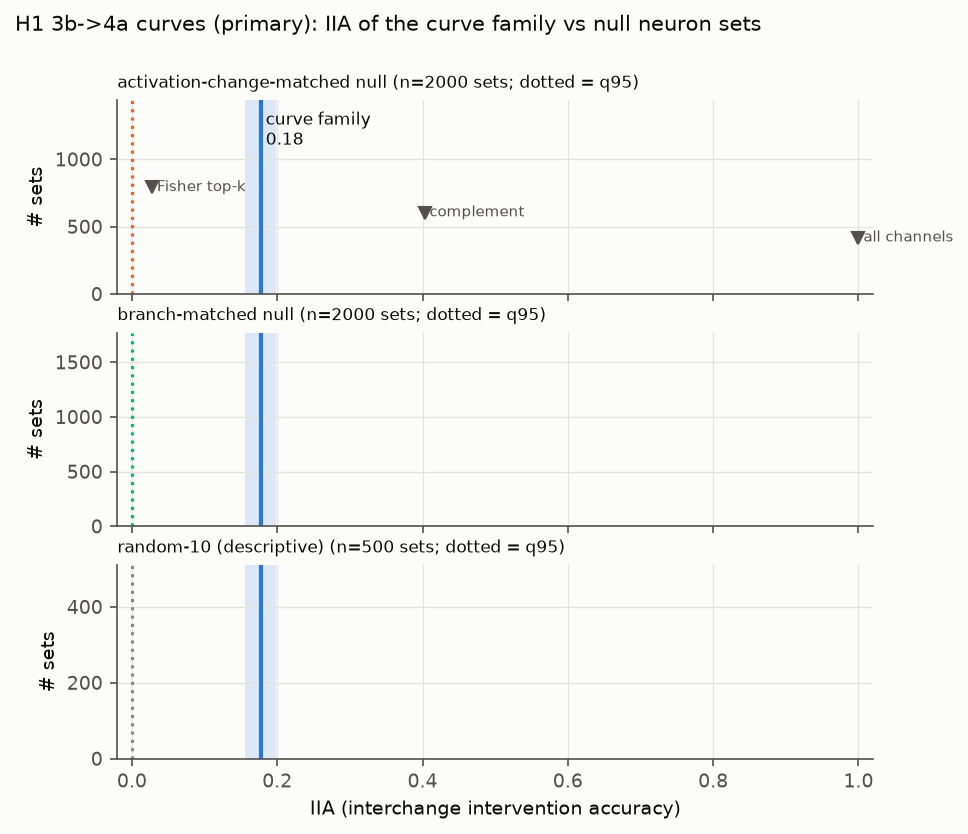
\includegraphics[width=0.49\linewidth]{e2_h1_iia_null.png}\hfill
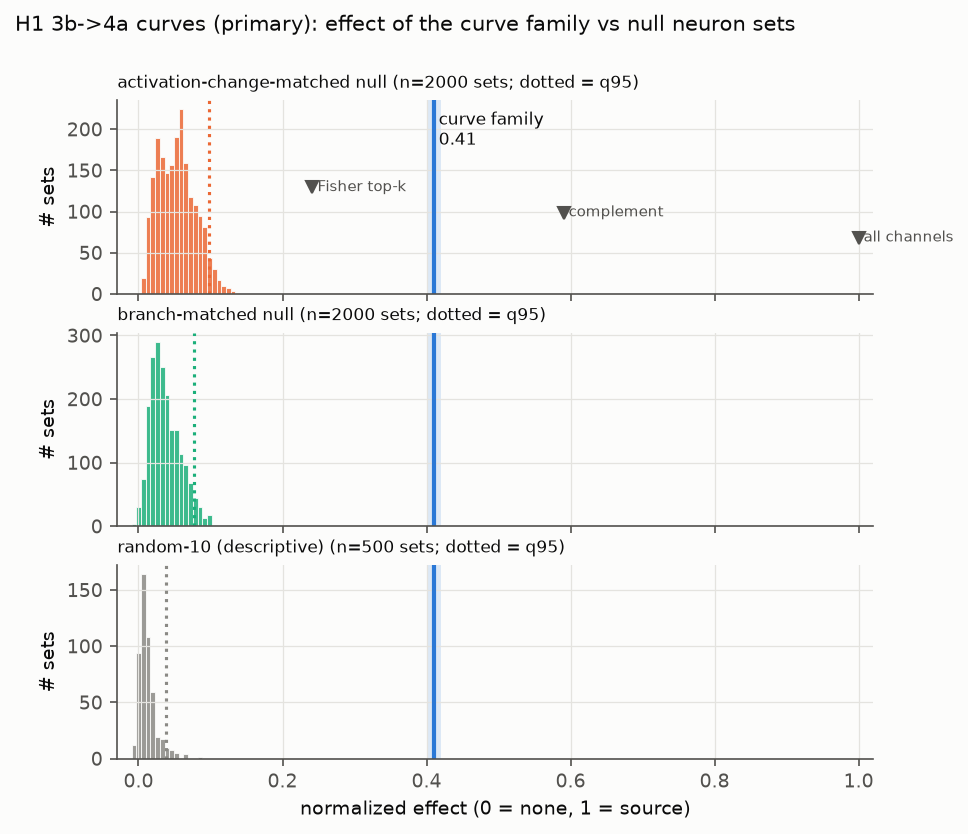
\includegraphics[width=0.49\linewidth]{e2_h1_effect_null.png}
\caption{H1. IIA (left) and normalized effect (right) of the curve family (blue line, 95\% CI band) against 2000 $\Delta$-matched, 2000 branch-matched and 500 random 10-channel null sets. Triangles mark the reference sets.}
\label{fig:h1}\end{figure}

\subsection{E3: natural images}
With arcs composited onto Imagenette photos, the H1 pattern recurs: $\iia=\HCompIIA$ and effect $\HCompEff$ against a null $q_{95}$ of $\HCompEffNullQ$. In the natural rotation counterfactual (H5) on $\HFiveNImg$ curve-present photos, the patched base is read as the rotated version in $\iia=\HFiveIIA$ of pairs. Its effect is $\HFiveEff$ against a null $q_{95}$ of $\HFiveEffNullQ$, while the complement dominates at $\iia=\HFiveCompl$. On curve-absent crops the family's effect halves to $\HFiveAbsentEff$ (exploratory). End to end, mean-ablating the family over the whole map changes the network's 1008-way top-1 prediction on $\RelFlipFam$ of $\RelN$ photos. Variance-matched null ablations change it on $\RelFlipNull$ ($q_{95}$ $\RelFlipQ$, $p=\RelFlipP$), and the mean KL is $\RelKLFam$ against $\RelKLNull$.

\subsection{Post-hoc robustness (not pre-registered)}
\label{sec:posthoc}
After the confirmatory run, an independent code review raised three ways the pre-registered comparisons could flatter the family. We tested each.
\begin{itemize}
\item \textbf{A softer-than-intended null.} All 10 curve units lie above the 96th percentile of activation change, so decile matching mostly draws channels that change less. A rank-matched null pairs each unit with one of its 10 nearest non-family channels by activation change (1000 sets). Against it, H1's effect $\PHOneEff$ still far exceeds the null $q_{95}$ of $\PHOneEffNullQ$. The 10 non-family channels with the largest activation change reach only $\PHOneTopEff$ and IIA $\PHOneTopIIA$. All other tests keep margin CIs above 0 (\texttt{reports/posthoc\_robustness.md}).
\item \textbf{Z-space vs decoded orientation.} Measured in the ridge decoder's $(\cos\theta,\sin\theta)$ output space, the family moves the decoded orientation vector $\PHRidgeCSEff$ of the way to the source's (rank-null $q_{95}$ $\PHRidgeCSRankQ$). It lands within $10^\circ$ in only $\HRidgeIIA$ of pairs, so the decoded orientation rotates only part of the way.
\item \textbf{Rotation blur in H5.} Rotating square crops by $-90/90/180^\circ$ is an exact transpose with no interpolation. Under these rotations the H5 effect is $\PHFiveExactEff$ (null $q_{95}$ $\PHFiveExactEffNullQ$) and IIA $\PHFiveExactIIA$, both larger than with the original, partly blurred rotations.
\end{itemize}

\begin{table}[t]\centering\small
\caption{Pre-registered tests. IIA and normalized effect of the curve family, with 95\% pigeonhole CIs, against the activation-change-matched null's $q_{95}$. Verdicts: H1 rows use the pre-registered three-way rule; the other rows use the secondary criterion (effect margin CI $>0$, Holm $p<0.05$). Full table: \texttt{reports/generated/results.md}.}
\label{tab:main}
\begin{tabular}{lcccl}\toprule
Test & IIA family & null $q_{95}$ & Effect (null $q_{95}$) & Verdict\\\midrule
H1: 3b$\to$4a curve units & \HOneIIA\ [\HOneIIALo, \HOneIIAHi] & \HOneNullQ & \HOneEff\ (\HOneEffNullQ) & \HOneVerdict\\
H1-ridge: 3b$\to$all 4a & \HRidgeIIA\ [\HRidgeIIALo, \HRidgeIIAHi] & \HRidgeNullQ & \HRidgeEff\ (\HRidgeEffNullQ) & \HRidgeVerdict\\
H2: curvature swap & \HTwoIIA\ [\HTwoIIALo, \HTwoIIAHi] & \HTwoNullQ & \HTwoEff\ (\HTwoEffNullQ) & \HTwoVerdict\\
H4: 3a$\to$3b curve units & \HFourIIA\ [\HFourIIALo, \HFourIIAHi] & \HFourNullQ & \HFourEff\ (\HFourEffNullQ) & \HFourVerdict\\
Composited (photos) & \HCompIIA\ [\HCompIIALo, \HCompIIAHi] & \HCompNullQ & \HCompEff\ (\HCompEffNullQ) & \HCompVerdict\\
H5: natural rotation & \HFiveIIA\ [\HFiveIIALo, \HFiveIIAHi] & \HFiveNullQ & \HFiveEff\ (\HFiveEffNullQ) & \HFiveVerdict\\
H1, jitter seed 3 & \HSeedThreeIIA\ [\HSeedThreeIIALo, \HSeedThreeIIAHi] & \HSeedThreeNullQ & \HSeedThreeEff\ (\HSeedThreeEffNullQ) & \HSeedThreeVerdict\\
H1, jitter seed 4 & \HSeedFourIIA\ [\HSeedFourIIALo, \HSeedFourIIAHi] & \HSeedFourNullQ & \HSeedFourEff\ (\HSeedFourEffNullQ) & \HSeedFourVerdict\\
H1, Lucent LRN & \HLrnIIA\ [\HLrnIIALo, \HLrnIIAHi] & \HLrnNullQ & \HLrnEff\ (\HLrnEffNullQ) & \HLrnVerdict\\\bottomrule
\end{tabular}\end{table}

\begin{figure}[t]\centering
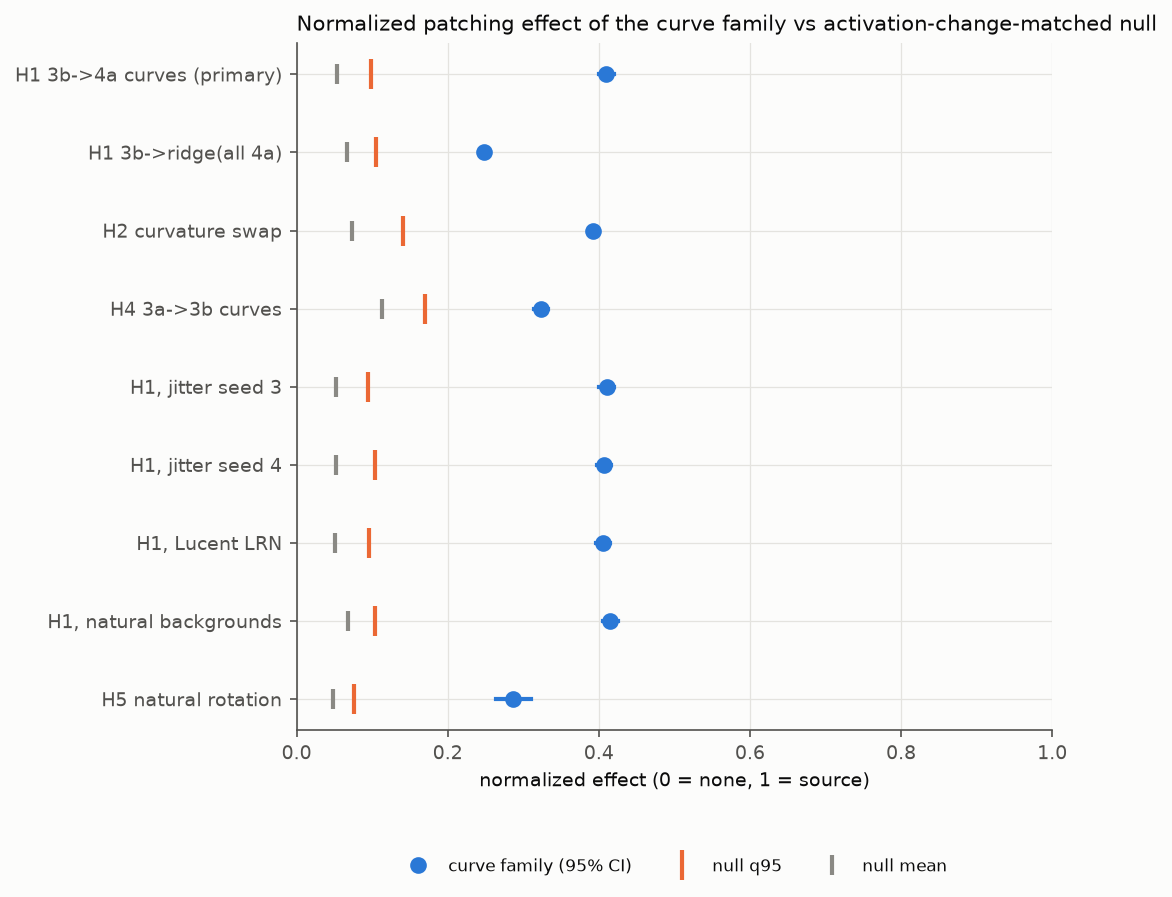
\includegraphics[width=0.8\linewidth]{summary_effect.png}
\caption{Normalized effect of the curve family (blue, 95\% CI) for every test, against the $\Delta$-matched null's mean (gray) and $q_{95}$ (orange).}
\label{fig:summary}\end{figure}

\section{Discussion}
\paragraph{What the explanation gets right.}
The Circuits description of the \texttt{mixed3b} curve units survives every observational check we ran. Interventions add something observation cannot show: the units are causally \emph{specific}. Among all 10-channel sets whose activations change as much between base and source, only the curve family moves the next layer's curve code substantially. It also carries curvature (H2), and removing it alters the network's decisions on natural images more than removing matched channels does.

\paragraph{What it gets wrong, or leaves out.}
The explanation is often read as ``these neurons are where the network represents curve orientation''. Under Huang et al.'s criterion, that reading fails: the family is not a sufficient mediator. Orientation is carried redundantly by many \texttt{mixed3b} channels, about 80 for reliable transfer. The family's contribution adds roughly linearly to theirs. This agrees with \citet{gorton2024missing}, who found curve features outside the 10 neurons, and with the language-model finding that single neurons rarely mediate concepts alone~\cite{huang2023rigorously}. In a causal-abstraction framing~\cite{geiger2023abstraction}, the orientation variable is realised by a distributed subspace of which the family is a privileged but partial part.

\paragraph{Implications.}
Neuron-level explanations in vision should be stated with an explicit causal scope. Two claims need separating: ``unit $u$ is selective for $X$'' (observational), and ``unit set $S$ mediates $X$ for downstream computation $Y$'' (interventional, with a stated readout). Activation-change-matched nulls are essential. Against random channels, almost any orientation-tuned set would look causally important, because most channels barely change between base and source.

\section{Limitations}
\begin{itemize}
\item \textbf{Single model and layer pair.} Only InceptionV1 and the 3b$\to$4a (and 3a$\to$3b) transition are tested. We do not claim generality to other CNNs or depths.
\item \textbf{Partly circular readout.} The primary readout uses curve units the authors relate to 3b curves. We mitigate this with a whole-layer ridge readout and natural-image tests, but both decoders are trained on clean data and judge patched, possibly off-manifold states. A same-orientation sham keeps the readout intact in $\HOneSham$ of pairs, which argues against patching artefacts, but it does not rule out decoder bias.
\item \textbf{Strict binary metric.} IIA needs the decoded orientation within 10$^\circ$ of the source. Partial transfer appears only in the continuous effect. The pre-registered rule judges H1 on IIA, which makes it a statement about strong sufficiency.
\item \textbf{Stimulus distribution.} The synthetic arcs are off-distribution for an ImageNet model. The composited and rotation experiments only partly address this. Rotating a photo changes far more than curve orientation, so H5's IIA is a conservative test.
\item \textbf{No learned subspaces.} We test the published neuron set, not an optimised mediator such as distributed alignment search~\cite{geiger2024das} or SAE features~\cite{gorton2024missing}. Whether a low-dimensional sufficient mediator exists is open.
\item \textbf{Bootstrap assumptions.} The pigeonhole bootstrap treats base and source as independent factors, although every image plays both roles, and it ignores clustering within the 16 jitter cells. In H2, lines at $\theta$ and $\theta+180^\circ$ are near-duplicates. Our CIs are therefore somewhat too narrow. The three jitter seeds agree to within 0.006 IIA, and no verdict is close to its threshold.
\item \textbf{Design details.} H5's clean decoding accuracy is 1.0 by construction, because its templates are the photo's own clean versions; success still requires the patched base to resemble the rotated version more than the unpatched base. The composited test reuses the same 32 backgrounds in both splits, so it generalises across jitter, not backgrounds. The 5\% denominator filter for the effect was computed over all pairs rather than only eligible ones, as the pre-registration states. At most 1.7\% of pairs are ineligible in any test (jitter seed 4), so the difference is negligible.
\item \textbf{Pilot disclosure.} The pilot already suggested IIA $\approx0.16$. Thresholds were not changed, and the pilot is disclosed in the pre-registration.
\end{itemize}

\section{Conclusion}
Counterfactual concept swaps turn the Circuits curve-detector explanation into a falsifiable causal claim. The claim splits into two parts. The ten \texttt{mixed3b} curve units are a \emph{specific} causal mediator of curve orientation and curvature: they far exceed activation-matched controls on synthetic and natural images and matter for the network's predictions. They are \emph{not} a sufficient one: swapping them alone transfers the decoded orientation in only \HOneIIA\ of pairs, because the code is distributed and redundant. We release the pre-registration, code, per-pair data and figures so these numbers can be checked and extended.


\bibliographystyle{plainnat}
\begin{thebibliography}{99}
\bibitem[Ameisen et~al.(2025)]{ameisen2025circuit} E.~Ameisen et al. Circuit tracing: Revealing computational graphs in language models. \emph{Transformer Circuits Thread}, 2025. \url{https://transformer-circuits.pub/2025/attribution-graphs/methods.html}
\bibitem[B{\"a}umel et~al.(2025)]{baeumel2025modular} T.~B{\"a}umel et al. Modular arithmetic: Language models solve math digit by digit. arXiv:2508.02513, 2025. \url{https://arxiv.org/abs/2508.02513}
\bibitem[Bau et~al.(2017)]{bau2017dissection} D.~Bau, B.~Zhou, A.~Khosla, A.~Oliva, A.~Torralba. Network dissection: Quantifying interpretability of deep visual representations. CVPR, 2017. \url{https://arxiv.org/abs/1704.05796}
\bibitem[Bau et~al.(2020)]{bau2020units} D.~Bau, J.-Y.~Zhu, H.~Strobelt, A.~Lapedriza, B.~Zhou, A.~Torralba. Understanding the role of individual units in a deep neural network. \emph{PNAS} 117(48):30071--30078, 2020. \url{https://doi.org/10.1073/pnas.1907375117}
\bibitem[Bricken et~al.(2023)]{bricken2023monosemanticity} T.~Bricken et al. Towards monosemanticity: Decomposing language models with dictionary learning. \emph{Transformer Circuits Thread}, 2023. \url{https://transformer-circuits.pub/2023/monosemantic-features}
\bibitem[Cammarata et~al.(2020)]{cammarata2020curve} N.~Cammarata, G.~Goh, S.~Carter, L.~Schubert, M.~Petrov, C.~Olah. Curve detectors. \emph{Distill}, 2020. \url{https://distill.pub/2020/circuits/curve-detectors/}
\bibitem[Cammarata et~al.(2021)]{cammarata2021circuits} N.~Cammarata, G.~Goh, S.~Carter, C.~Voss, L.~Schubert, C.~Olah. Curve circuits. \emph{Distill}, 2021. \url{https://distill.pub/2020/circuits/curve-circuits/}
\bibitem[Cammarata(2026)]{cammarata2026clean} N.~Cammarata. Neural networks are already clean. Goodfire, 2026. \url{https://already-clean.goodfire.com/}
\bibitem[Chan et~al.(2022)]{chan2022scrubbing} L.~Chan et al. Causal scrubbing: a method for rigorously testing interpretability hypotheses. Alignment Forum, 2022. \url{https://www.alignmentforum.org/posts/JvZhhzycHu2Yd57RN/causal-scrubbing-a-method-for-rigorously-testing}
\bibitem[ICML(2026)]{colorneurons2026} A critical analysis of color neurons in vision models. ICML, 2026. \url{https://icml.cc/virtual/2026/79523}
\bibitem[Geiger et~al.(2021)]{geiger2021causal} A.~Geiger, H.~Lu, T.~Icard, C.~Potts. Causal abstractions of neural networks. NeurIPS, 2021. \url{https://arxiv.org/abs/2106.02997}
\bibitem[Geiger et~al.(2023)]{geiger2023abstraction} A.~Geiger et al. Causal abstraction: A theoretical foundation for mechanistic interpretability. arXiv:2301.04709, 2023. \url{https://arxiv.org/abs/2301.04709}
\bibitem[Geirhos et~al.(2023)]{geirhos2023trust} R.~Geirhos et al. Don't trust your eyes: on the (un)reliability of feature visualizations. arXiv:2306.04719, 2023. \url{https://arxiv.org/abs/2306.04719}
\bibitem[Geiger et~al.(2024)]{geiger2024das} A.~Geiger, Z.~Wu, C.~Potts, T.~Icard, N.~Goodman. Finding alignments between interpretable causal variables and distributed neural representations. CLeaR, 2024. \url{https://arxiv.org/abs/2303.02536}
\bibitem[Gorton(2024)]{gorton2024missing} L.~Gorton. The missing curve detectors of InceptionV1: Applying sparse autoencoders to InceptionV1 early vision. arXiv:2406.03662, 2024. \url{https://arxiv.org/abs/2406.03662}
\bibitem[Gu et~al.(2011)]{gu2011fisher} Q.~Gu, Z.~Li, J.~Han. Generalized Fisher score for feature selection. UAI, 2011. \url{https://arxiv.org/abs/1202.3725}
\bibitem[Gurnee et~al.(2026)]{gurnee2026workspace} W.~Gurnee, N.~Sofroniew, et al., J.~Lindsey. Verbalizable representations form a global workspace in language models. \emph{Transformer Circuits Thread}, 2026. transformer-circuits.pub/2026/workspace.
\bibitem[Heimersheim and Nanda(2024)]{heimersheim2024patching} S.~Heimersheim, N.~Nanda. How to use and interpret activation patching. arXiv:2404.15255, 2024. \url{https://arxiv.org/abs/2404.15255}
\bibitem[Huang et~al.(2023)]{huang2023rigorously} J.~Huang, A.~Geiger, K.~D'Oosterlinck, Z.~Wu, C.~Potts. Rigorously assessing natural language explanations of neurons. BlackboxNLP, 2023. \url{https://arxiv.org/abs/2309.10312}
\bibitem[Kopf et~al.(2024)]{kopf2024cosy} L.~Kopf et al. CoSy: Evaluating textual explanations of neurons. NeurIPS, 2024. \url{https://arxiv.org/abs/2405.20331}
\bibitem[Leavitt and Morcos(2020)]{leavitt2020selectivity} M.~L.~Leavitt, A.~S.~Morcos. Selectivity considered harmful: evaluating the causal impact of class selectivity in DNNs. arXiv:2003.01262, 2020. \url{https://arxiv.org/abs/2003.01262}
\bibitem[Luo et~al.(2016)]{luo2016erf} W.~Luo, Y.~Li, R.~Urtasun, R.~Zemel. Understanding the effective receptive field in deep convolutional neural networks. NeurIPS, 2016. \url{https://arxiv.org/abs/1701.04128}
\bibitem[Morcos et~al.(2018)]{morcos2018single} A.~S.~Morcos, D.~G.~T.~Barrett, N.~C.~Rabinowitz, M.~Botvinick. On the importance of single directions for generalization. ICLR, 2018. \url{https://arxiv.org/abs/1803.06959}
\bibitem[Oikarinen et~al.(2025)]{oikarinen2025evaluating} T.~Oikarinen, G.~Yan, T.-W.~Weng. Evaluating neuron explanations: A unified framework with sanity checks. ICML, 2025. \url{https://arxiv.org/abs/2506.05774}
\bibitem[Olah et~al.(2020a)]{olah2020zoom} C.~Olah, N.~Cammarata, L.~Schubert, G.~Goh, M.~Petrov, S.~Carter. Zoom in: An introduction to circuits. \emph{Distill}, 2020. \url{https://distill.pub/2020/circuits/zoom-in/}
\bibitem[Olah et~al.(2020b)]{olah2020early} C.~Olah, N.~Cammarata, L.~Schubert, G.~Goh, M.~Petrov, S.~Carter. An overview of early vision in InceptionV1. \emph{Distill}, 2020. \url{https://distill.pub/2020/circuits/early-vision/}
\bibitem[Olah et~al.(2020c)]{olah2020equivariance} C.~Olah, N.~Cammarata, C.~Voss, L.~Schubert, G.~Goh. Naturally occurring equivariance in neural networks. \emph{Distill}, 2020. \url{https://distill.pub/2020/circuits/equivariance/}
\bibitem[Owen(2007)]{owen2007pigeonhole} A.~B.~Owen. The pigeonhole bootstrap. \emph{Annals of Applied Statistics} 1(2):386--411, 2007. \url{https://doi.org/10.1214/07-AOAS122}
\bibitem[Phipson and Smyth(2010)]{phipson2010permutation} B.~Phipson, G.~K.~Smyth. Permutation p-values should never be zero. \emph{Stat.\ Appl.\ Genet.\ Mol.\ Biol.} 9(1):39, 2010. \url{https://doi.org/10.2202/1544-6115.1585}
\bibitem[Szegedy et~al.(2015)]{szegedy2015going} C.~Szegedy et al. Going deeper with convolutions. CVPR, 2015. \url{https://arxiv.org/abs/1409.4842}
\bibitem[Voss et~al.(2021)]{voss2021branch} C.~Voss et al. Branch specialization. \emph{Distill}, 2021. \url{https://distill.pub/2020/circuits/branch-specialization/}
\bibitem[Zhang and Nanda(2024)]{zhang2024patching} F.~Zhang, N.~Nanda. Towards best practices of activation patching in language models: Metrics and methods. ICLR, 2024. \url{https://arxiv.org/abs/2309.16042}
\end{thebibliography}

\appendix
\section{Reproducibility and statistics details}
Code, tests and the pre-registration are at \url{https://github.com/BurnyCoder/counterfactually-causal-analysis-of-convolutional-neural-networks-with-concept-swaps}. Per-pair data are in the Hugging Face dataset \url{https://huggingface.co/datasets/BurnyCoder/inceptionv1-curve-concept-swaps}. All numbers in this paper are \LaTeX\ macros generated from the result files (\texttt{reports/generated/numbers.tex}).

Runtime is about one hour on an RTX~5070 Laptop GPU. Determinism: TF32 is disabled, and stimuli, pairs and null sets are seeded. The cropped-window recomputation equals the full network in fp64 to $10^{-14}$.

Null sizes: 2000 per null for H1 and H4; 1000 for H2, the composited test and H5; 500 for the ridge readout, the seeds and the LRN check. The smallest attainable permutation $p$ is $1/(M+1)$.

Deviations from the approved plan are listed in the pre-registration: the planned locality hypothesis became a unit test, and the secondary decision criterion was specified before the confirmatory run.

\section{Exploratory results}
IIA by $|\Delta\theta|$ bin (30--60, 60--90, 90--120, 120--150, 150--180$^\circ$): \DThetaA, \DThetaB, \DThetaC, \DThetaD, \DThetaE. H5 IIA by rotation angle: \HFiveIIAFortyFive\ at $+45^\circ$ and \HFiveIIAOneEighty\ at 180$^\circ$.

\begin{figure}[h]\centering
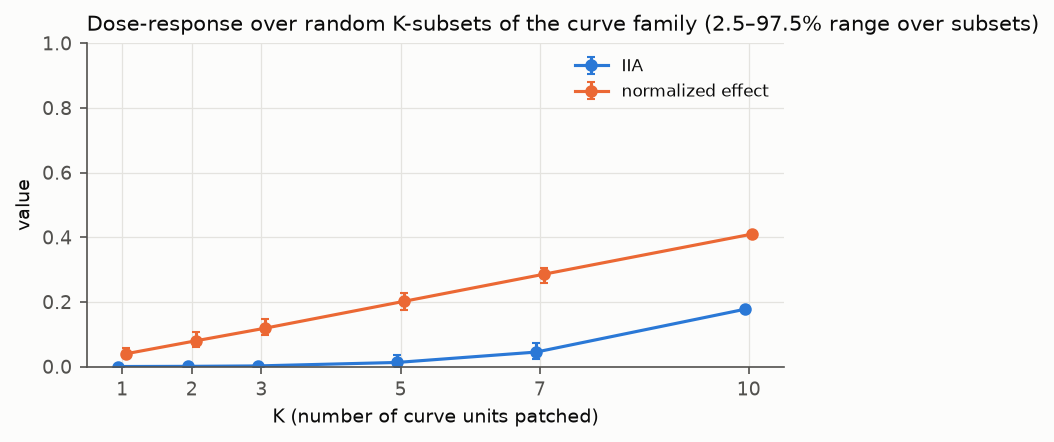
\includegraphics[width=0.49\linewidth]{e2_h1_dose.png}\hfill
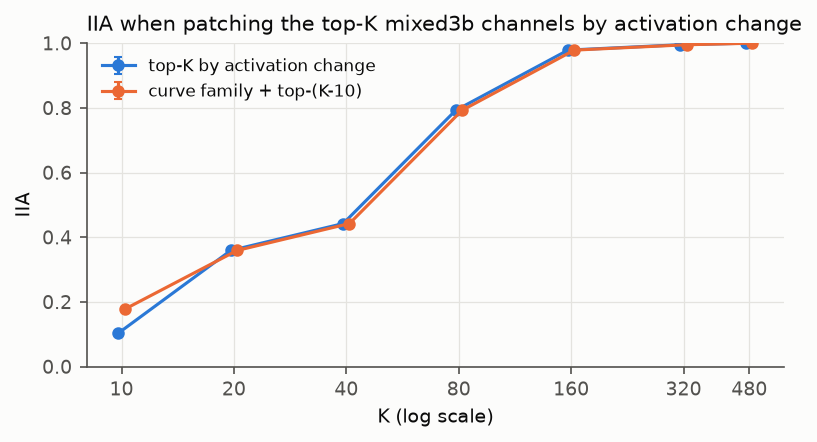
\includegraphics[width=0.49\linewidth]{e2_h1_topk.png}
\caption{Left: dose-response over random $K$-subsets of the curve family. Right: IIA when patching the top-$K$ \texttt{mixed3b} channels by activation change; the $x$ axis shows $\log_2K$.}
\end{figure}

\section*{AI statement}
This codebase and paper were written by Claude Code (Anthropic's coding agent, model Claude Opus 5.5). Libor Burian provided the exact research idea that Claude Code executed: counterfactual concept-swap interventions validating a Circuits neuron explanation in a CNN. Human cleanup and rewriting are in progress.

\end{document}
